\chapter{Análise de Resultados}
\label{chap:analise}

\section{Fotometria das amostras}

A combinação dos doze filtros e a fotometria de diferentes aberturas do S-PLUS (Figuras \ref{fig:filtroscartwheel} e \ref {fig:am0417391}), desempenham um papel fundamental na visualização de dados astronômicos e na realização de uma ampla gama de estudos científicos, por exemplo, obter informações de propriedades das populações estelares como idade e metalicidade, que necessitariam de espectroscopia. A qualidade fotométrica dos \emph{surveys} é importante para a ciência que se aplica a estes dados.

\begin{figure}[!h]
    \centering 
    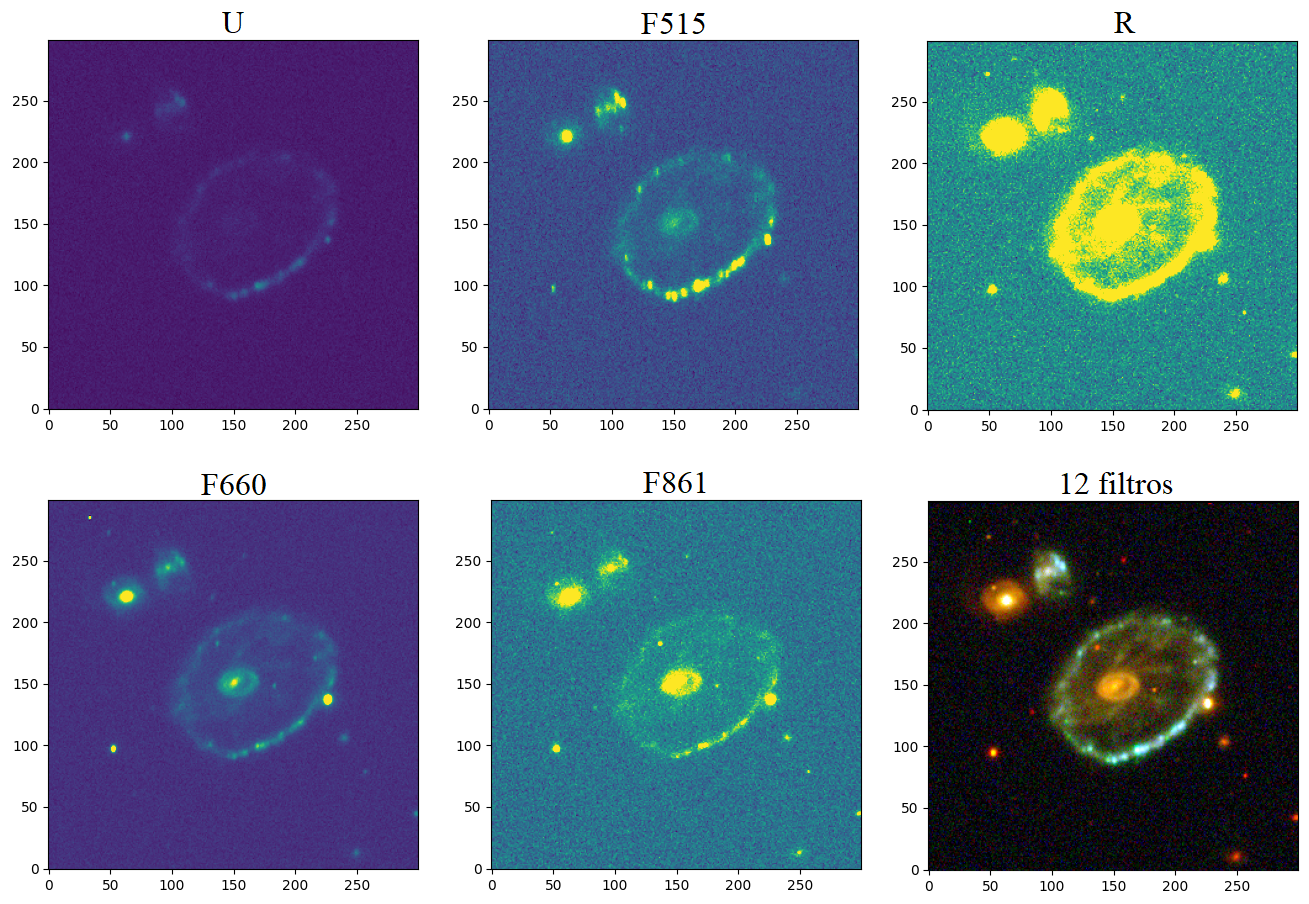
\includegraphics[width=0.9\textwidth]{Imagens/filtroscartwheel.png} 
    \caption[Filtros individuais e combinados de AM 0035-335.]{Observa-se na galáxia AM 0035-335 pelas intensidades das cores, as concentrações e distribuições das estrelas e as características das regiões do bojo e dos anéis, interno e externo. O anel externo, elíptico, amplo e com nódulos possui uma tonalidade azulada, com estrelas jovens da população 1. O bojo e o anel interno, mais avermelhado, com estrelas mais velhas da população 2. Podemos ver também, vários ``raios'' ligandos os anéis, como uma possível trilha evolutiva de estrelas.}
    \label{fig:filtroscartwheel} 
\end{figure}

Podemos observar, através da combinação dos doze filtros (Figura \ref{fig:exemplos_dozefiltros}), a riqueza de informações sobre as galáxias de nossa amostra, como as características elípticas ou circulares dos anéis, presença de un anel interno próximo ao bojo (núcleo), diversas cores que as estrelas apresentam, refletindo suas diferentes idades, e também regiões de concentração de poeira e gás. Em particular, o filtro J0660 (H$\alpha$) é satisfatório para estudar hidrogênio até desvios para o vermelho de z $\approx$ 0.015, ferramenta importante para medir a taxa de formação estelar \cite{2022MNRAS.511.4590A}. Mas qual a qualidade fotométrica para estes objetos peculiares? Devido a sua morfologia irregular, anéis extensos, interação em andamento e efeitos tidais, é essencial verificar a fotometria de abertura nos objetos, e se as aberturas elípticas são confiáveis para nossa amostra.

\begin{figure}[!h]
  \centering 
  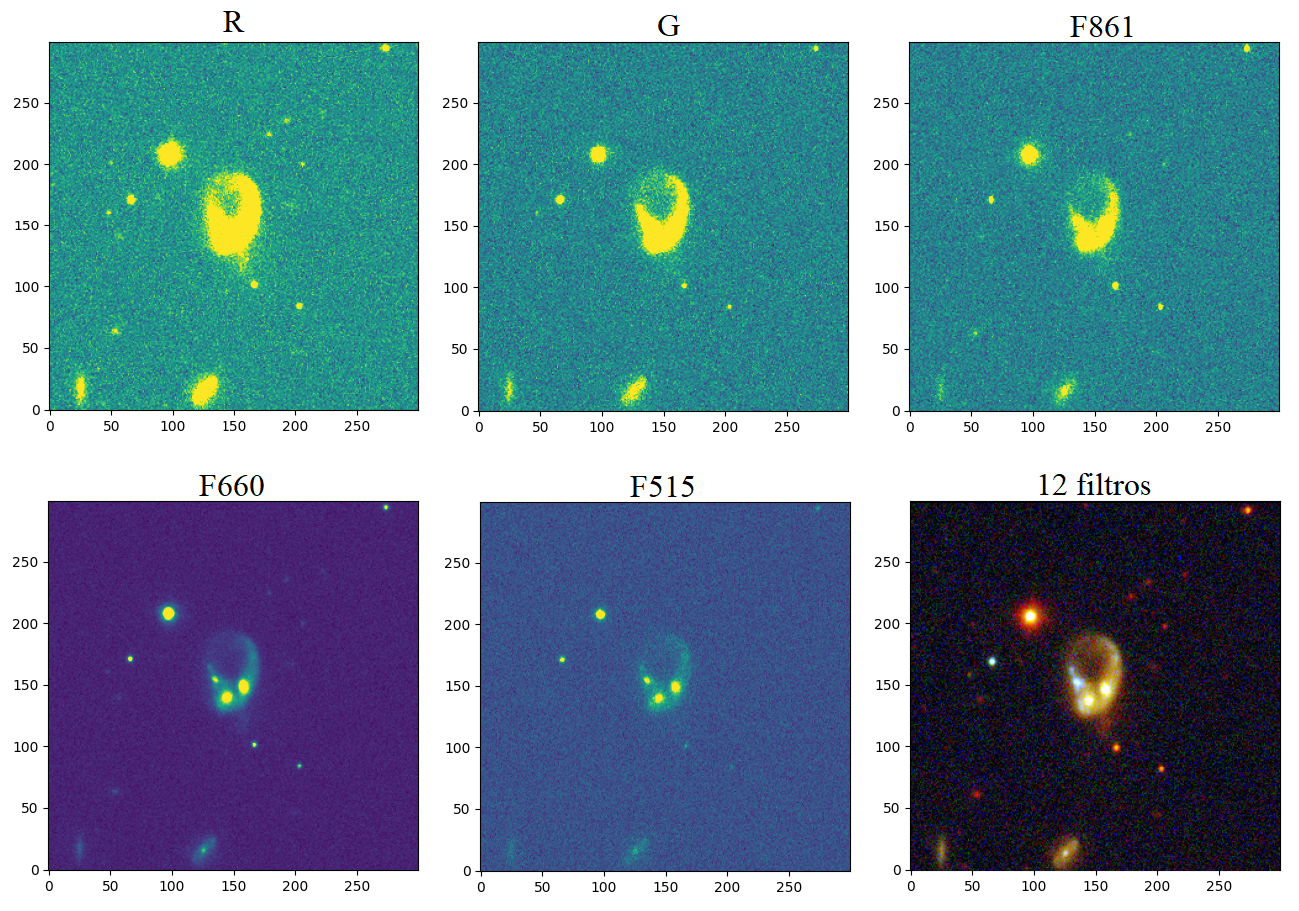
\includegraphics[width=0.9\textwidth]{Imagens/am0417391.png}
  \caption[Filtros individuais e combinados de AM 0417-391.]{A galáxia AM 0417-391, resultado da colisão entre duas galáxias, exibe nódulos marcantes no anel, não apresentando bojo na região central nem deslocado.}
  \label{fig:am0417391}
\end{figure}

\begin{figure}[!h]
  \centering 
  \includegraphics[width=0.95\textwidth]{Imagens/exemplos_dozefiltros.png} 
  \caption[Exemplos de galáxias aneladas peculiares pela combinação de doze filtros do S-PLUS.]{Exemplos de galáxias de nossa amostra observadas através da combinação de doze filtros do S-PLUS. Podemos ver as diversas formas e peculiaridades dos anéis e suas particulares características, e identificar suas famílias de acordo com a classificação de \citeonline{1998abans}.}
  \label{fig:exemplos_dozefiltros} 
\end{figure}

\begin{figure}[!h]
  \centering 
  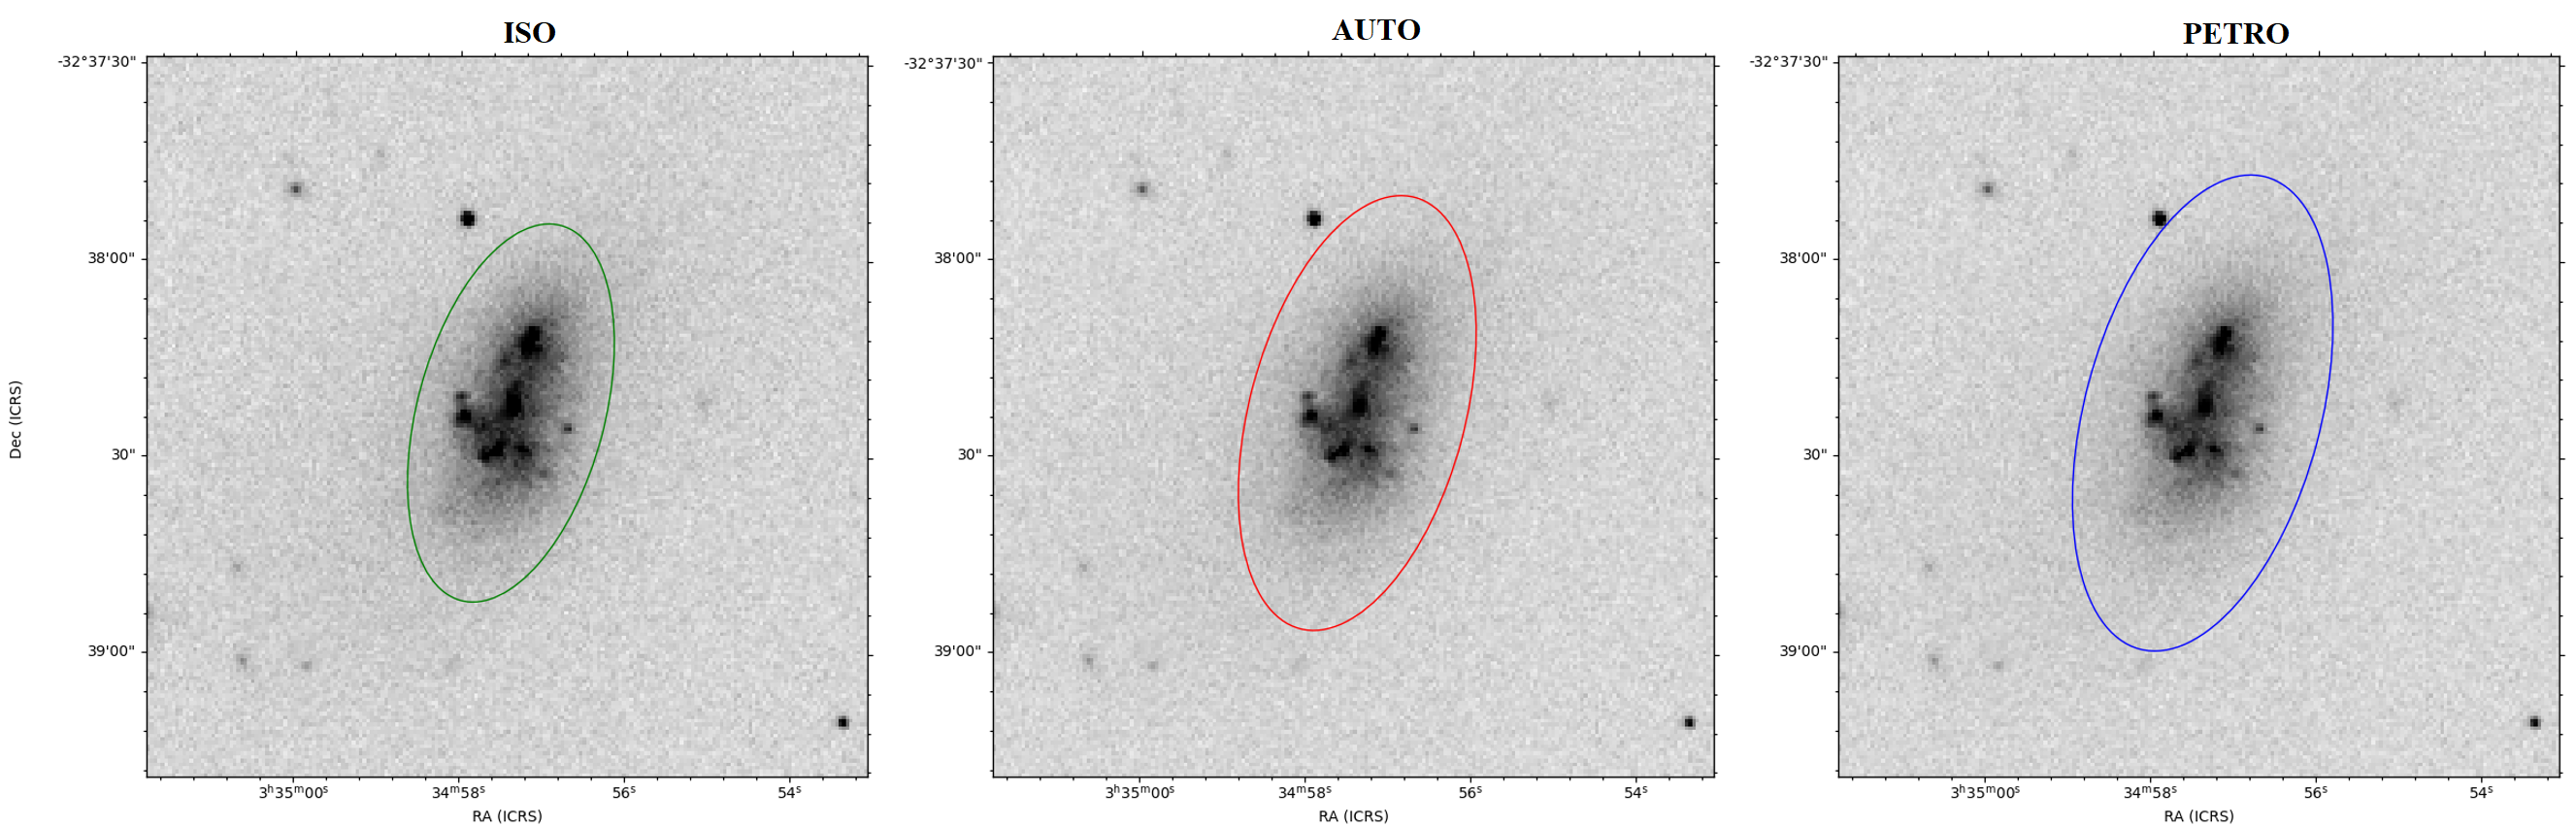
\includegraphics[width=1.0\textwidth]{Imagens/aberturas_am0332324.png} 
  \caption[Aberturas aplicadas à galáxia AM 0332-324.]{Galáxia AM 0332-324 vista com o filtro H$\alpha$: observa-se que as três aberturas elípticas abrangem bem a galáxia.}
  \label{fig:aberturas_am0332324} 
\end{figure}

\begin{figure}
  \centering 
  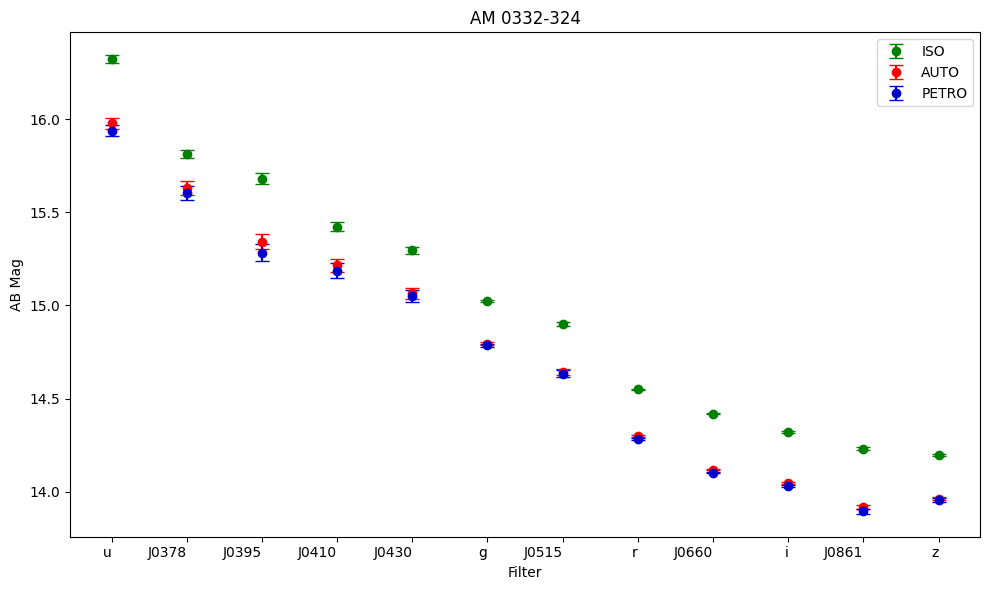
\includegraphics[width=1.0\textwidth]{Imagens/am0332324barraerro.png} 
  \caption[AM 0332-324: magnitudes em cada abertura para os 12 filtros.]{Galáxia AM 0332-324: visualização da leitura das magnitudes em cada abertura para os 12 filtros e suas respectivas barras de erro.}
  \label{fig:am0332324barraerro} 
\end{figure}

As tabelas obtidas do S-PLUS contêm dados de todas as fontes detectáveis na imagem. Portanto, foi necessário remover as elipses que não faziam parte do nosso objeto de estudo, a fim de nos concentrarmos nos dados de nosso interesse. Isso foi feito ao analisar as informações de cada linha das tabelas e selecionar apenas os dados referentes à nossa galáxia. Para algumas galáxias (Figura \ref{fig:aberturas_am0332324}) as aberturas parecem abranger bem seus formatos, logo, podemos dizer que a fotometria é confiável, e desta forma, somos capazes de analisar as informações de suas magnitudes e fluxos para todos os filtros, comparando qualidade de leitura para cada abertura, e também, realizar a distribuição espectral de energia (a partir dos dados fotométricos, temos apenas uma visão de como seria o espectro da galáxia, porém, para afirmarmos tais propriedades, é necessário realizar espectroscopia) (Figura \ref{fig:am0332324barraerro}); para outras (Figuras \ref{fig:aberturas_am0058311}), não podemos concordar. Nossa amostra foi dividida em dois grupos, as 61 galáxias que possuem qualidade fotométrica para as três aberturas (elipse envolve todo o objeto) e as 51 que não possuem. Com esse cenário, analisamos os dados para cada filtro, comparando as barras de erro e características como os diferentes formatos de bojo e anéis, em virtude da importância dos doze filtros que o S-PLUS possui.

\begin{figure}[h]
  \centering 
  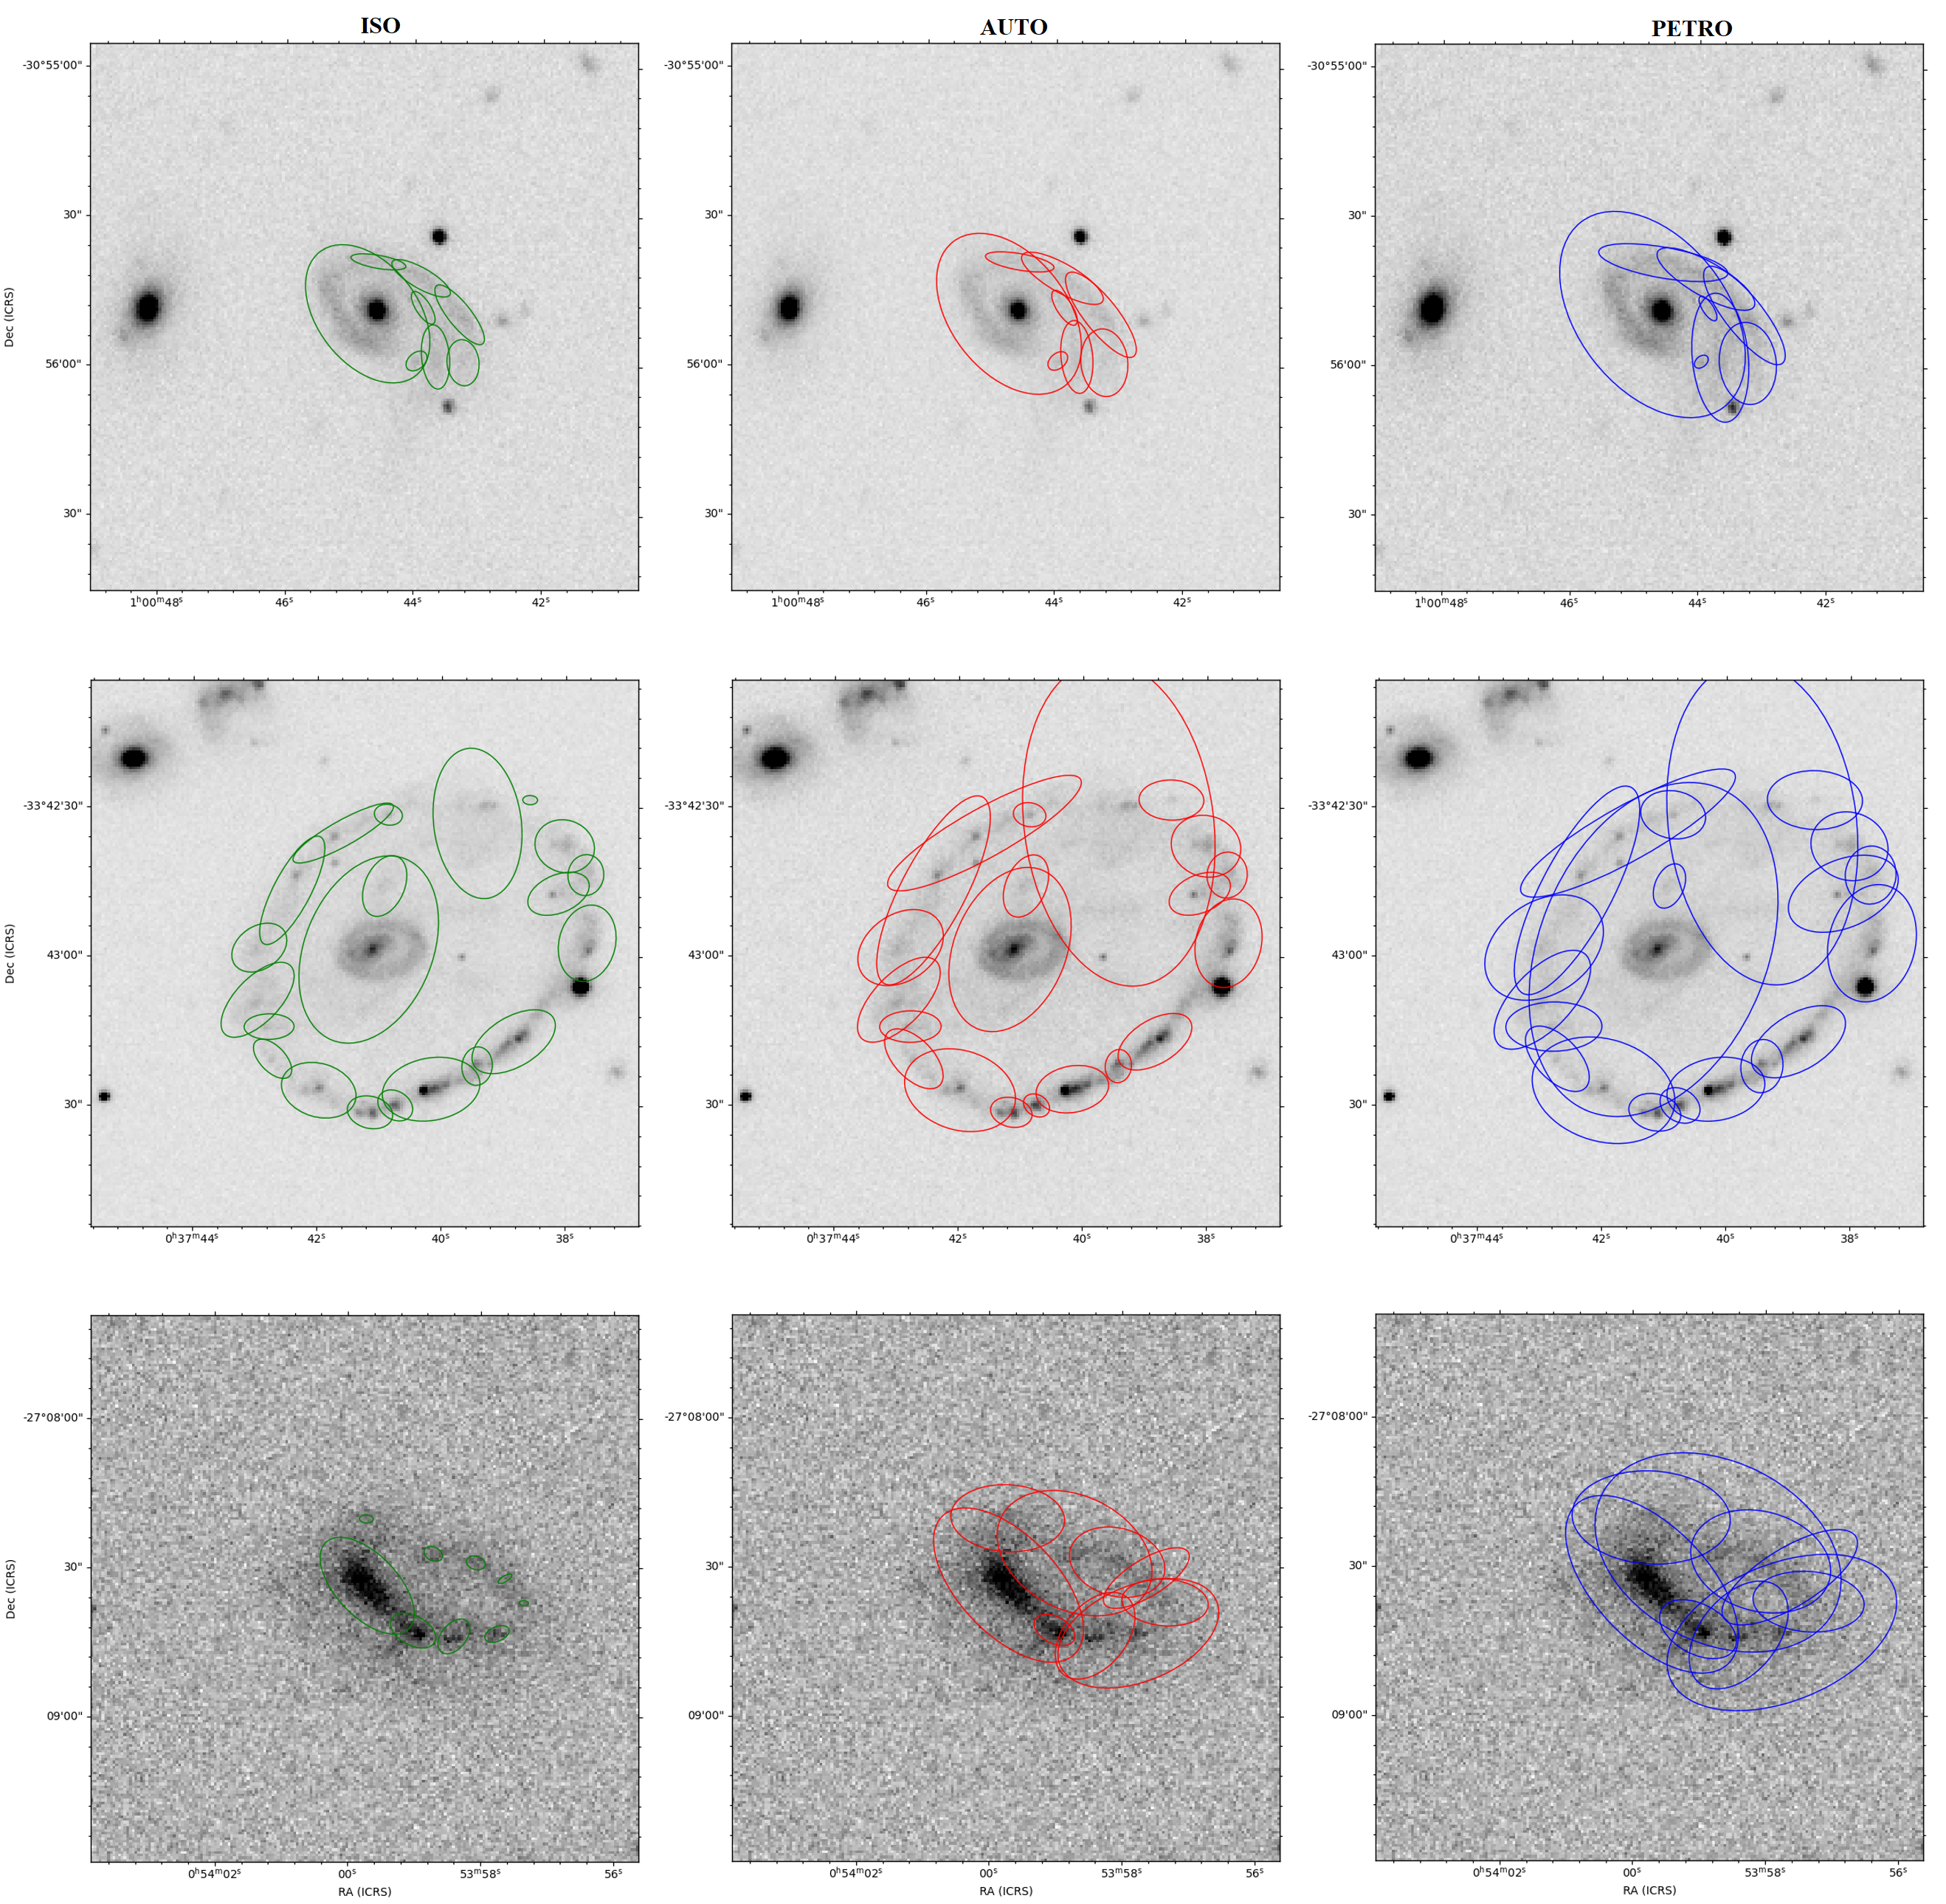
\includegraphics[width=1.0\textwidth]{Imagens/aberturas_am0058311.png} 
  \caption[Aberturas aplicadas à galáxia AM 0058-311.]{Galáxia AM 0058-311 vista com o filtro R: para as três aberturas é possível ver várias leituras de partes da galáxia, logo, conseguimos informações dessas regiões separadas, e não do objeto como um todo.}
  \label{fig:aberturas_am0058311} 
\end{figure}

Vimos que não podemos apenas obter os dados fotométricos das aberturas e gerar os gráficos sem antes realizar uma análise individual de nossas galáxias. Essa análise parte da busca das informações nas tabelas disponíveis pelo banco de dados do S-PLUS. Como mencionado, a busca é pelas coordenadas RA e DEC de cada objeto e traz informações de todas as fontes detectáveis para cada foto. Logo, para um objeto mais extenso, com caudas de maré ou outras peculiaridades (como os anéis), outros píxeis de detecção são calculados com elipses separadas da elipse da galáxia. Isso se deve à exatidão do algoritmo do SExtractor para um corpo extenso. Assim, para estes objetos, apenas as informações presentes na linha específica da coordenada RA e DEC da galáxia na tabela, traz somente os dados de uma região, ou seja, uma parte da galáxia (como mostra a Figura \ref{fig:aberturas_am0058311}).

Dois exemplos para a análise dos dados fotométricos são observados nas Figuras \ref{fig:A03364905} e \ref{fig:AM0330324}, que são galáxia mais difusas e com cores diferentes entre si, e seus respectivos gráficos, que representa para a galáxia A 03364905, que a fotometria ilustra bem as características observáveis (Figura \ref{fig:A03364905exemplo}) e para a AM 0330-324, temos informações separadas de partes da galáxia (Figuras \ref{fig:AM0330324index16}, \ref{fig:AM0330324index4} e \ref{fig:AM0330324index9}).

\begin{figure}[!h]
  \centering 
  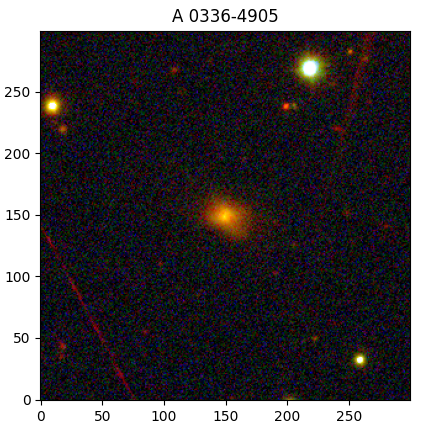
\includegraphics[width=0.4\textwidth]{Imagens/A03364905.png} 
  \caption[Galáxia A 03364905 (Anon 0336-4905) com a combinação dos doze filtros.]{Visualização da galáxia A 03364905 (Anon 0336-4905) (e Figura \ref{fig:A03364905exemplo}) com os doze filtros. Ela possui uma coloração predominantemente vermelha.}
  \label{fig:A03364905} 
\end{figure}

\begin{figure}[h]
  \centering 
  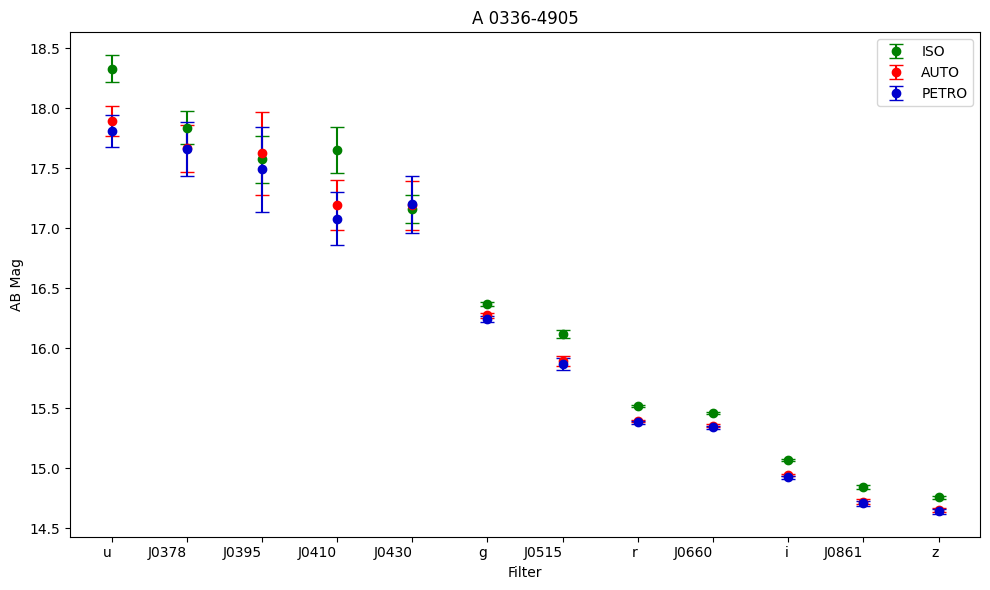
\includegraphics[width=0.8\textwidth]{Imagens/A03364905exemplo.png} 
  \caption[Magnitudes da galáxia A 03364905 (Anon 0336-4905).]{Esta galáxia possui qualidade fotométricapara todos os filtros. Podemos observar destaque em H$\alpha$ e as metalicidades J0861 (tripleto de Ca) e J0515 (tripleto de Mgb), provenientes de estrelas jovens, e \emph{riz} realçando estrelas velhas e poeira interestelar.}
  \label{fig:A03364905exemplo} 
\end{figure}

\begin{figure}[h]
  \centering 
  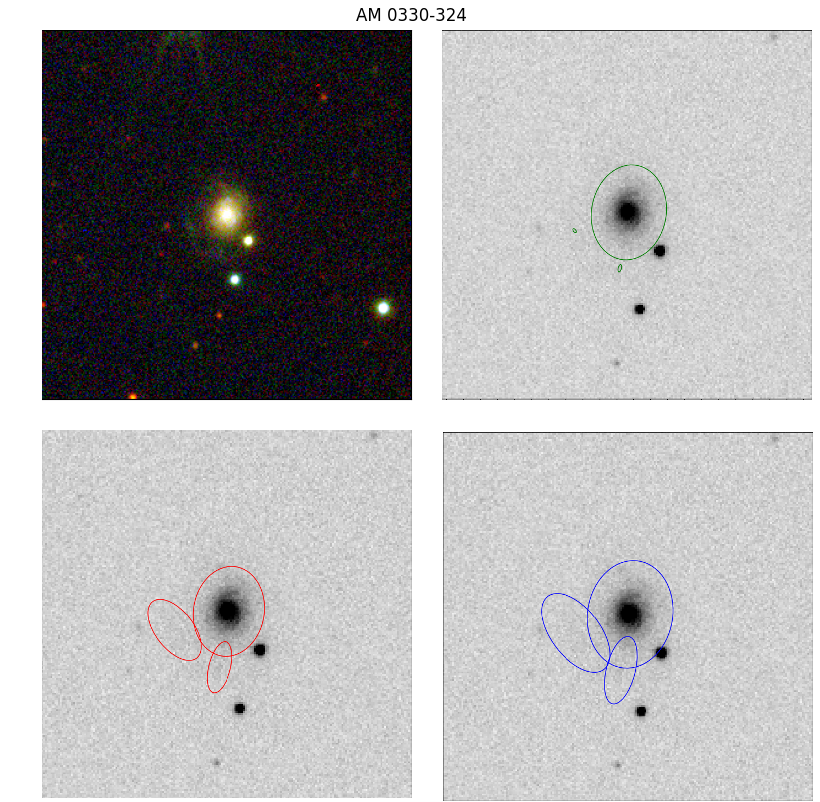
\includegraphics[width=0.4\textwidth]{Imagens/AM0330324.png} 
  \caption[Galáxia AM 0330-324 com a combinação dos doze filtros.]{Visualização da galáxia AM 0330-324 (e Figuras \ref{fig:AM0330324index16}, \ref{fig:AM0330324index4} e \ref{fig:AM0330324index9}) com os doze filtros. Ela apresenta um suave anel difuso e um bojo proeminente no anel.}
  \label{fig:AM0330324} 
\end{figure}

\begin{figure}[!h]
  \centering 
  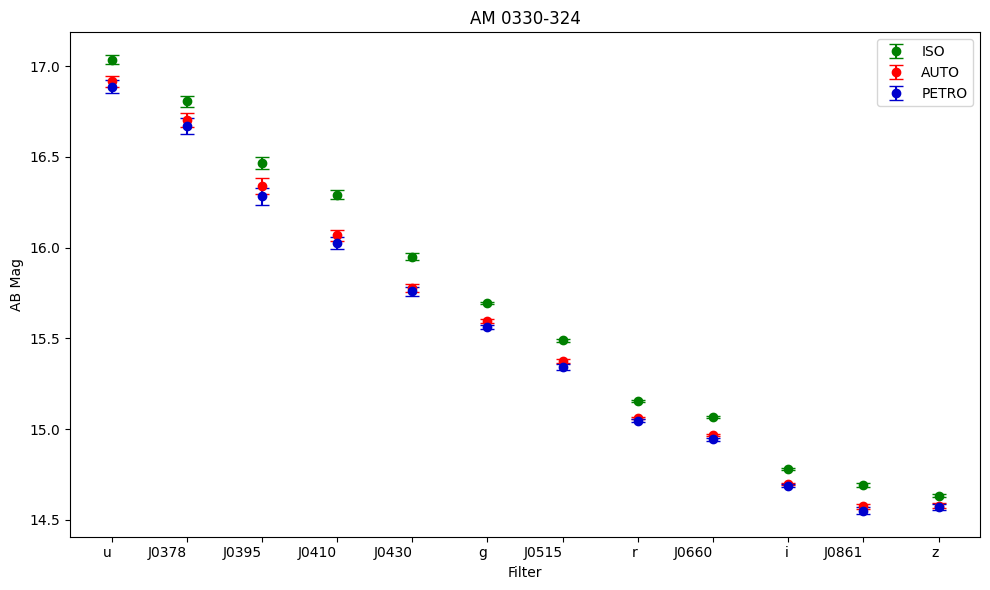
\includegraphics[width=0.8\textwidth]{Imagens/AM0330324index16.png} 
  \caption[Magnitudes da galáxia AM 0330-324.]{Esta galáxia é um exemplo de fotometria não confiável, pois possui leitura de magnitudes de três regiões (elipses): bojo e duas regiões no anel. Este gráfico representa a área do bojo.}
  \label{fig:AM0330324index16} 
\end{figure}

\begin{figure}[!h]
  \centering 
  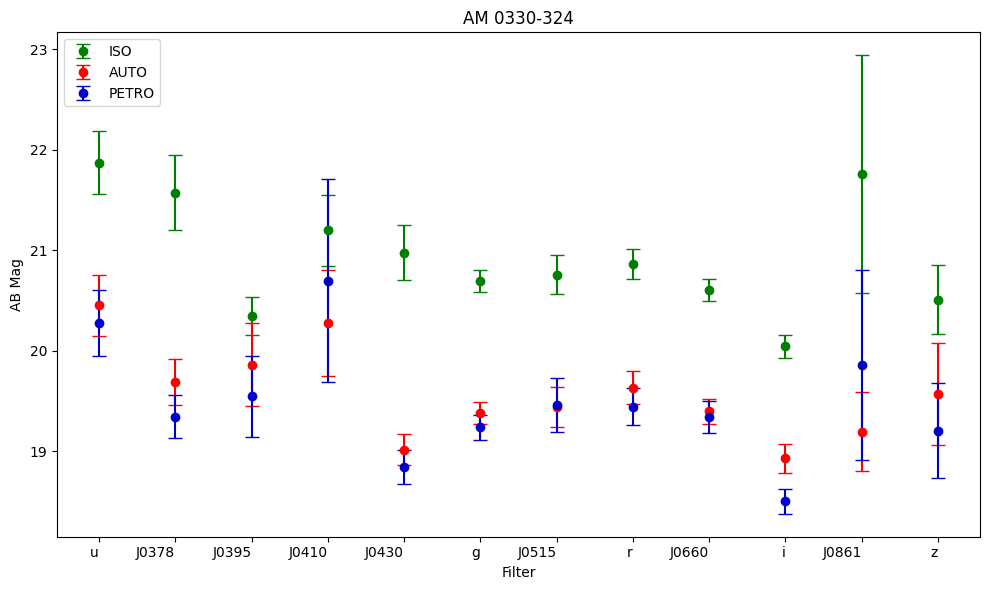
\includegraphics[width=0.8\textwidth]{Imagens/AM0330324index4.png} 
  \caption[Magnitudes da galáxia AM 0330-324.]{Este gráfico representa uma região do anel difuso, logo, há maior barra de erro na leitura das magnitudes.}
  \label{fig:AM0330324index4} 
\end{figure}

\begin{figure}[!h]
  \centering 
  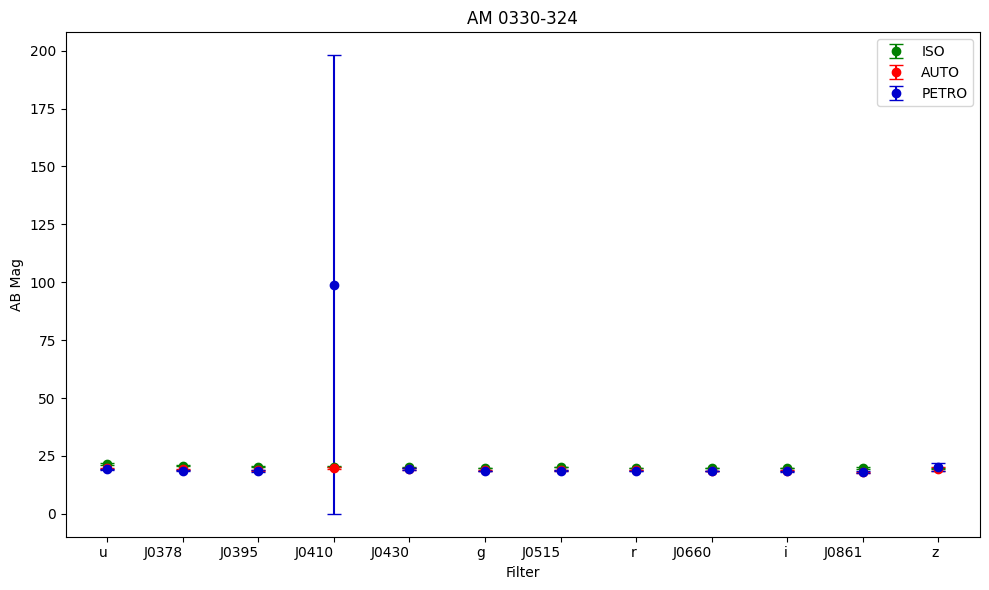
\includegraphics[width=0.8\textwidth]{Imagens/AM0330324index9.png} 
  \caption[Magnitudes da galáxia AM 0330-324.]{Este gráfico mostra a segunda região do anel. Por ser uma região muito difusa, percebe-se que a abertura PETRO para o filtro J0410 (H$\delta$) não faz leitura da magnitude, representado por um valor extrapolado.}
  \label{fig:AM0330324index9} 
\end{figure}

\begin{figure}[h]
  \centering 
  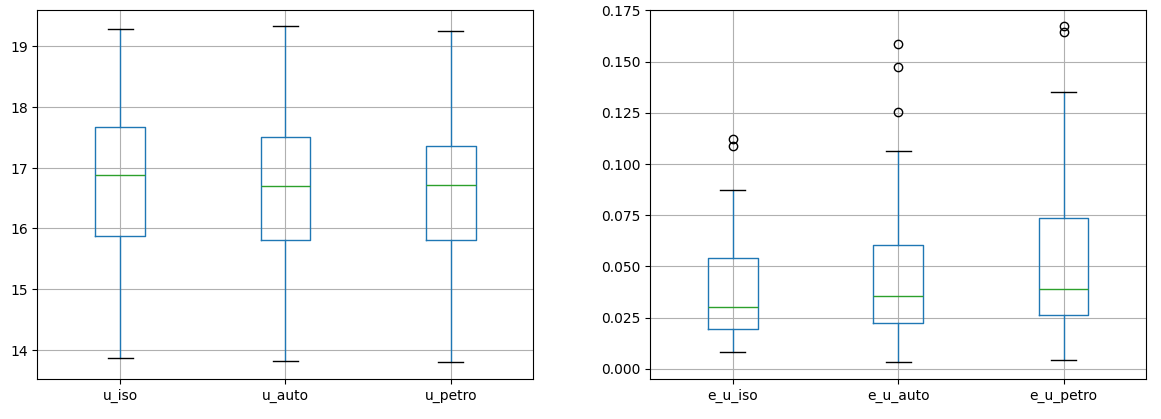
\includegraphics[width=1.0\textwidth]{Imagens/boxplot_aberturas_err.png}
  \caption[Distribuição dos valores das magnitudes e respectivos erros pela representação gráfica \emph{boxplot} e identificação de dados extrapolados para o filtro U.]{Representação gráfica da distribuição dos valores das magnitudes (esquerda) e respectivos erros (direita) para o filtro U. A linha verde dentro do retângulo representa a mediana (valor que divide os dados em duas metades iguais); a região abaixo e acima da mediana dentro do retângulo são respectivamente o primeiro quartil (valor que separa os 25\% valores inferiores do restante) e terceiro quartil (valor que separa os 25\% valores superiores dos dados do restante); e whiskers (linhas que se estendem a partir do retângulo até os valores extremos dentro de 1.5 vezes a diferença entre terceiro e primeiro quartil). Os dados fora da faixa whiskers são considerados outliers e são mostrados como pontos individuais.}
  \label{fig:boxplot_aberturas} 
\end{figure}

Para as galáxias que as aberturas fotométricas são confiáveis, 61 objetos representados na Figura \ref{fig:galaxias}, retiramos as medidas extrapoladas (exemplo de extrapolação na Figura \ref{fig:AM0330324index9}), simbolizadas pelo valor 99 nas tabelas, e comparamos as barras de erro na medição das magnitudes entre elas (Figura \ref{fig:incerteza_abertura}). Para esta separação de dados dos objetos que possuem algum tipo de extrapolação, foi utilizada a ferramenta de representação gráfica \emph{boxplot} (Figura \ref{fig:boxplot_aberturas}), que utiliza da distribuição dos valores de um conjunto de dados, para identificar a presença de \emph{outliers} (pontos de dados que se afastam significativamente da maioria dos outros pontos em um conjunto de dados), sendo a maioria destes, os valores representados por 99 pelas tabelas do S-PLUS, e avaliar a dispersão dos dados (identificação de padrões ou discrepâncias significativas). Analisando os dados para as três aberturas, percebe-se que a ISO tem uma medição de magnitude ligeiramente maior que a AUTO e PETRO, e uma menor barra de erro. A PETRO possui uma medição menor que as outras duas aberturas, porém, com maior barra de erro (como observado na Figura \ref{fig:galaxias}).

\begin{figure}[!h]
  \centering 
  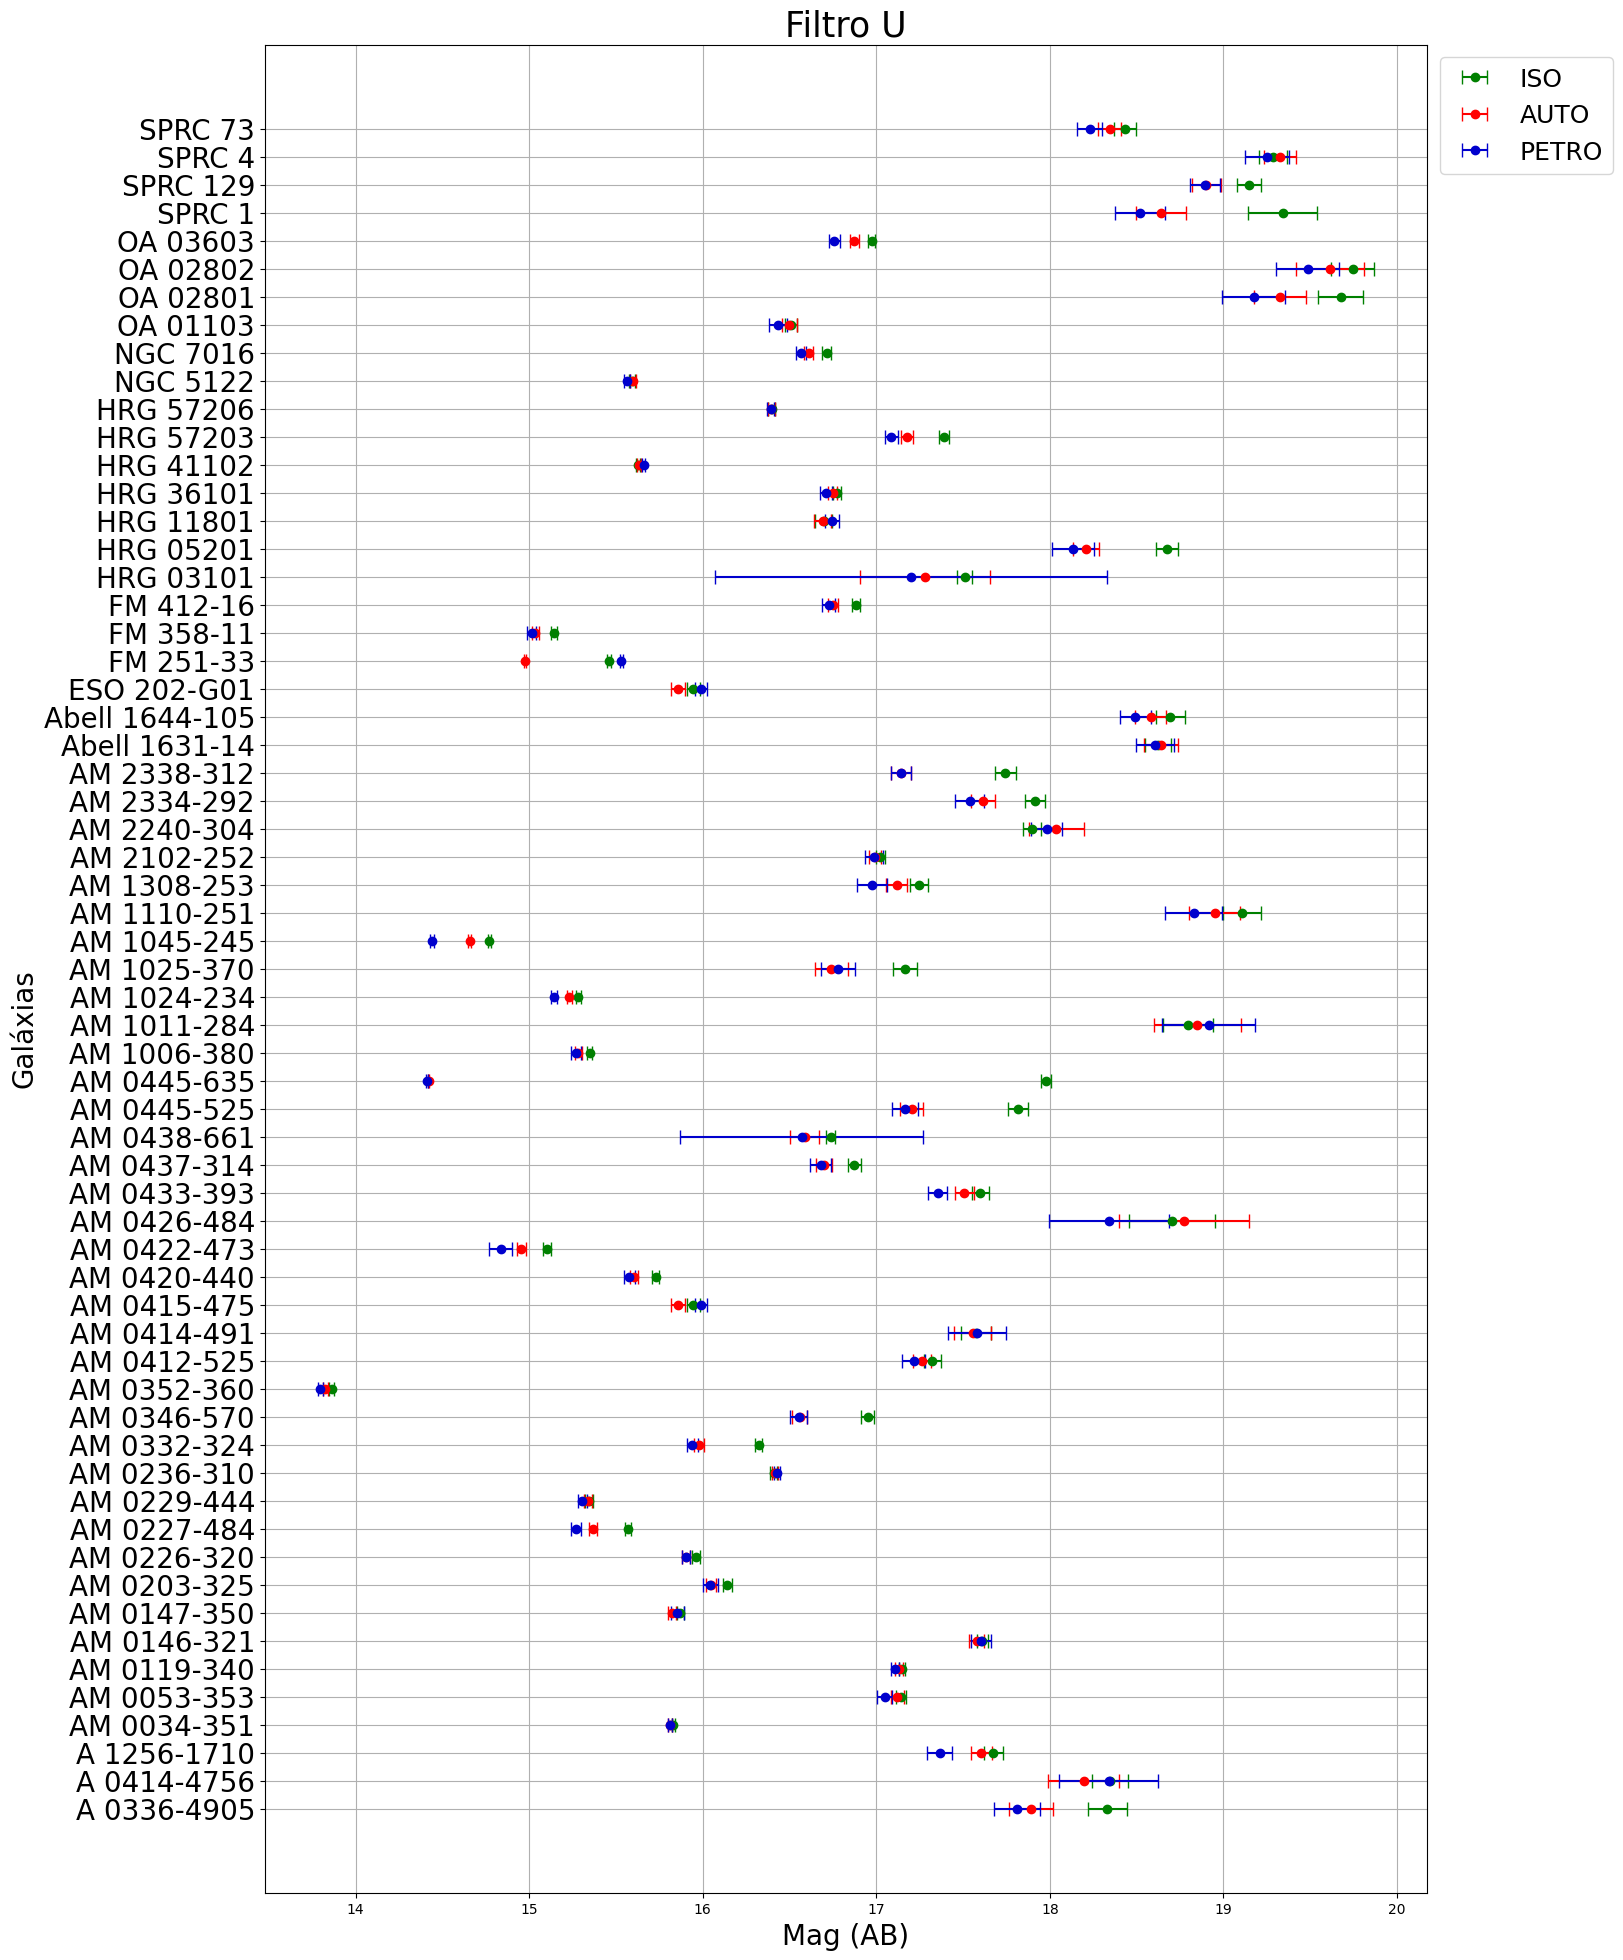
\includegraphics[width=1.0\textwidth]{Imagens/galaxias_vertical.png}
  \caption[Nossa amostra vista em todos os filtros para as três aberturas fotométricas.]{Característica de nossa amostra de galáxias para as três aberturas fotométricas, onde se observa que as medições de magnitudes são ligeiramente diferentes e algumas possuem barras de erro maiores que outras.}
  \label{fig:galaxias} 
\end{figure}

\begin{figure}[h]
  \centering 
  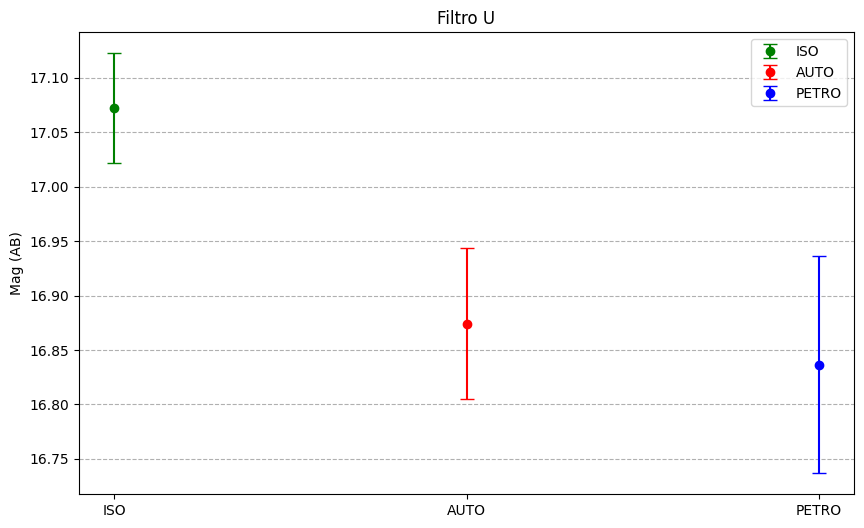
\includegraphics[width=0.8\textwidth]{Imagens/incerteza_abertura.png} 
  \caption[Média entre as três aberturas e seus respectivos erros para o filtro U.]{Representação da média entre as magnitudes e entre as barras de erro do filtro U para as 61 galáxias em que as aberturas abragem todo o corpo do objeto. Para esta análise, todas as medições extrapoladas foram retiradas.}
  \label{fig:incerteza_abertura} 
\end{figure}

Uma outra visão comparativa entre as medições das três aberturas foi realizada em relação aos valores das magnitudes, como mostram as Figuras \ref{fig:iso_auto}, \ref{fig:iso_petro} e \ref{fig:auto_petro}. Observa-se nessas imagens que quanto maior a magnitude do objeto (ou seja, menor seu brilho), maior será a probabilidade da barra de erro. Nas Figuras \ref{fig:iso_linear}, \ref{fig:auto_linear} e \ref{fig:petro_linear}, temos a combinação do gráfico de dispersão com uma linha de regressão (modela a relação entre a magnitude e o erro) e histogramas marginais direita e superior (representa a distribuição da ``magnitude'' e ``erro'' individualmente), onde podemos observar uma dispersão maior nas medições AUTO e ISO, e um agrupamento maior e ``linear'' para a PETRO. Uma interpretação provável seria que para magnitudes menores que 18 mag, as aberturas AUTO e ISO sejam melhores, e para magnitudes maiores que 18 mag, a abertura PETRO seja mais confiável. 

\begin{figure}
  \centering 
  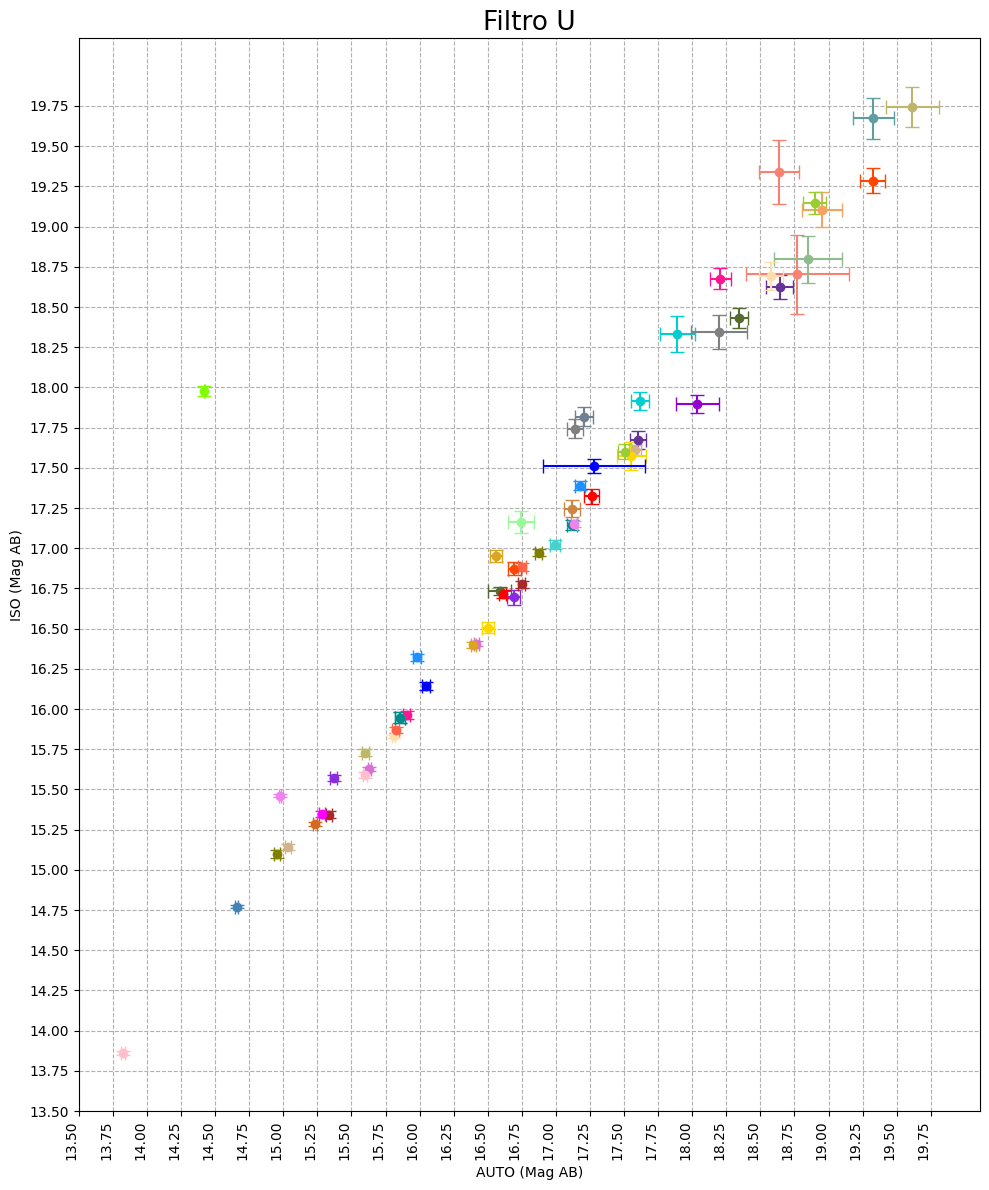
\includegraphics[width=0.7\textwidth]{Imagens/iso_auto.png} 
  \caption[Relação entre magnitudes e barras de erro para ISO e AUTO no filtro U.]{Relação entre magnitudes e barras de erro para ISO e AUTO no filtro U.}
  \label{fig:iso_auto} 
\end{figure}

\begin{figure}
  \centering 
  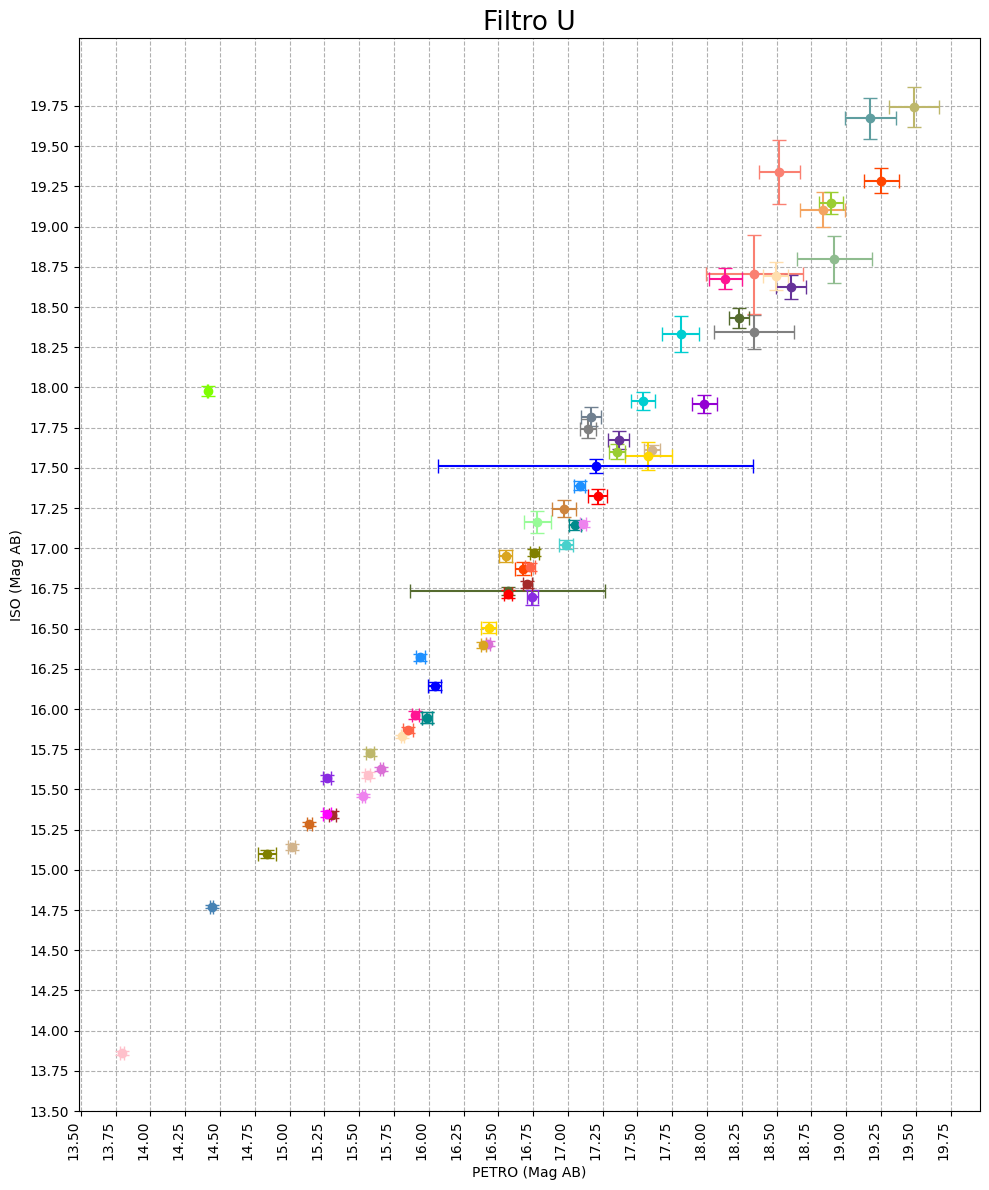
\includegraphics[width=0.7\textwidth]{Imagens/iso_petro.png} 
  \caption[Relação entre magnitudes e barras de erro para ISO e PETRO no filtro U.]{Relação entre magnitudes e barras de erro para ISO e PETRO no filtro U.}
  \label{fig:iso_petro}
\end{figure}

\begin{figure}
  \centering 
  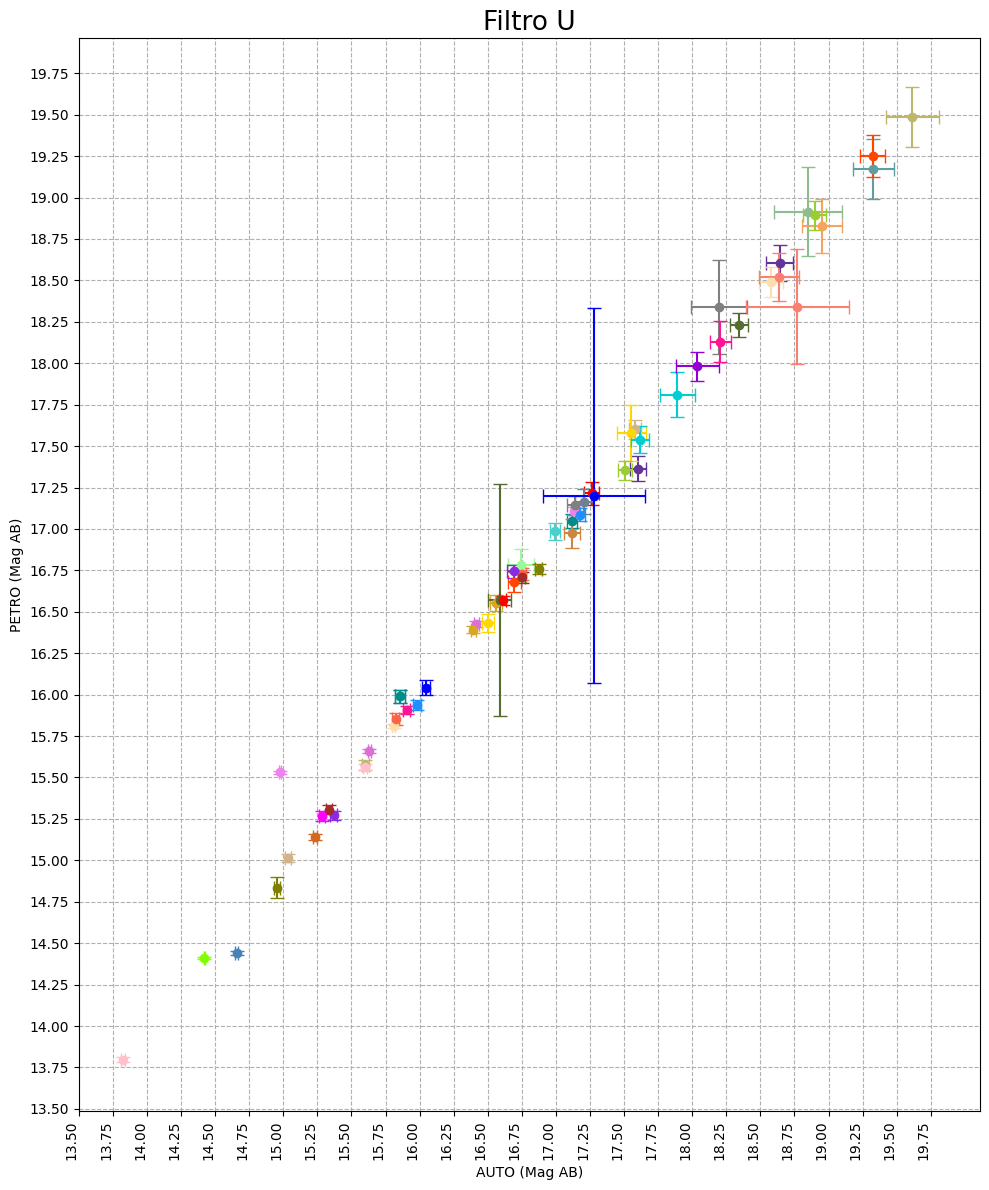
\includegraphics[width=0.7\textwidth]{Imagens/auto_petro.png} 
  \caption[Relação entre magnitudes e barras de erro para PETRO e AUTO no filtro U.]{Relação entre magnitudes e barras de erro para PETRO e AUTO no filtro U.}
  \label{fig:auto_petro} 
\end{figure}

\begin{figure}
  \centering 
  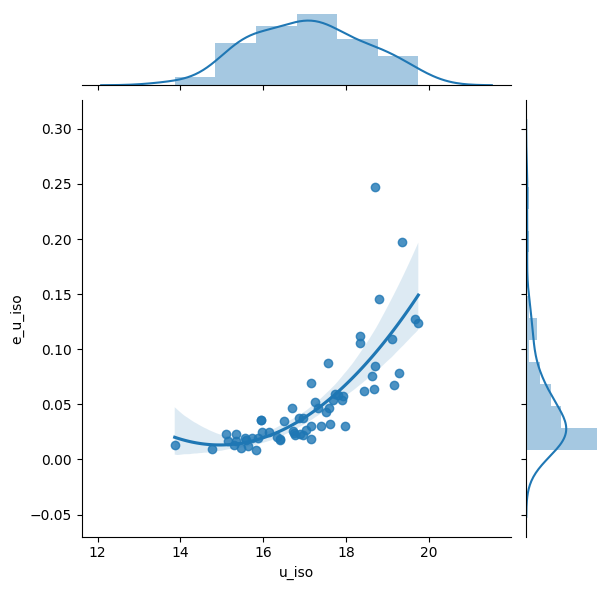
\includegraphics[width=0.6\textwidth]{Imagens/iso_linear.png} 
  \caption[Agrupamento das galáxias em relação à medição da magnitude e erro para a abertura ISO no filtro U.]{Para o filtro U, observa-se uma dispersão maior no agrupamento dos dados na abertura ISO.}
  \label{fig:iso_linear} 
\end{figure}

\begin{figure}
  \centering 
  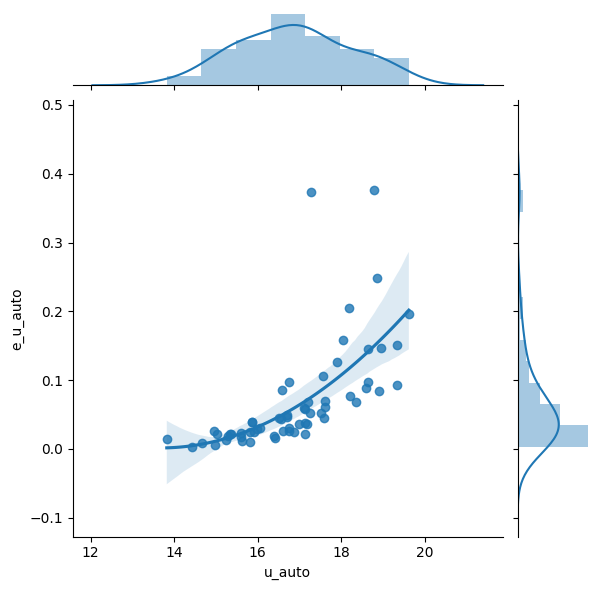
\includegraphics[width=0.6\textwidth]{Imagens/auto_linear.png} 
  \caption[Agrupamento das galáxias em relação à medição da magnitude e erro para a abertura AUTO no filtro U.]{Para o filtro U, observa-se também uma dispersão maior no agrupamento dos dados na abertura AUTO.}
  \label{fig:auto_linear} 
\end{figure}

\begin{figure}[t]
  \centering 
  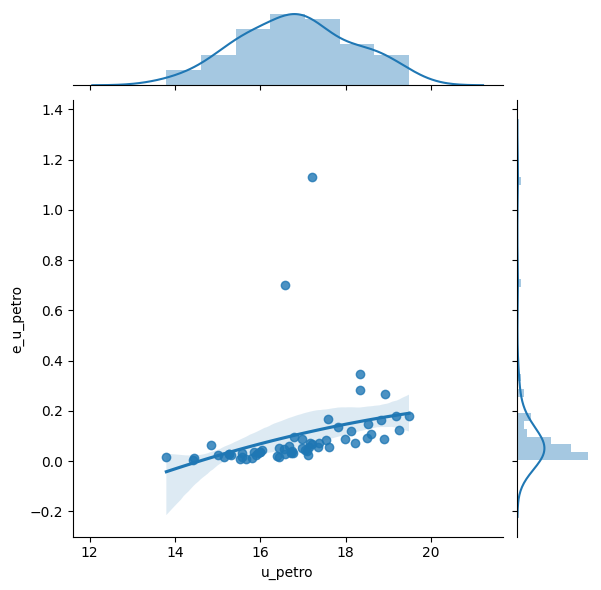
\includegraphics[width=0.6\textwidth]{Imagens/petro_linear.png} 
  \caption[Agrupamento das galáxias em relação à medição da magnitude e erro para a abertura PETRO no filtro U.]{Para o filtro U, observa-se uma dispersão menor no agrupamento dos dados na abertura PETRO.}
  \label{fig:petro_linear} 
\end{figure}